% Shared by both versions: the sparse (hashed-position) profile, moved out
% of the body. The full version includes it in appendix-eval.tex, the short
% version in appendix-compare.tex. The body keeps one sentence (body-tree.tex).
% Sizes are from spec/scripts/sizes.md; the 2^16 exit at D = 32 is measured
% (tools/test_scripts.py, test_exit_sparse_large) and set once in main.tex as \sparseExitBig.

\subsection{The Sparse Profile}\label{app:sparse}

In the sparse profile a leaf's position is the low $D$ bits of
$\Hpos(\mathsf{owner\_key} \,\|\, \mathsf{nonce})$, so the tree is the
Merkle-sum sparse Merkle tree of Taproot Assets~\cite{mssmt} truncated to
$D = 32$ or $64$. Direction bits are derived in script from the position
hash, and empty siblings are elided from the witness (the script
substitutes $\Emp_k$), so the witness grows with $\log_2 N$ rather than
with $D$. A sparse position is a function of the leaf: a joiner computes it
alone, a key and nonce cannot appear twice, the root depends only on the
leaf set, and absence is an inclusion proof of $\Emp_0$. None of
LayerTree's predicates needs these properties. An exit proves inclusion
and a join proves that its slot is $\Emp_h$, the same way in both profiles.
The dense profile has aligned subtrees instead, on which \tr{JOIN}$_h$,
\tr{EVICT\_SUBTREE}$_h$ and every batch shape depend, so the sparse
profile cannot graft or sweep and batches only by \tr{JOINK}$_K$. It still
hosts channel leaves and vouchers and still exits in one transaction.

\paragraph{Where the bytes go.} A sparse proof is the smaller witness and
the larger script, and the script wins (Table~\ref{tab:sparse}). Both
causes follow from hashing the position. Random positions collide, with
$N^2/2^{D+1}$ expected collisions among $N$ members (about one half at
$D = 32$ for $N = 2^{16}$, about 32{,}000 at $D = 16$), so the sparse tree
needs about twice the depth, and every level is unrolled. A sparse level
is also 135 bytes of script against 88, because it derives the direction
bit from the position, substitutes $\Emp_k$ for an elided sibling and
computes $\Emp_{k+1}$ for the next level. The full-width tree of Taproot
Assets ($D = 256$) costs $35{,}611$ bytes of script per exit, about 17
times the dense script and 9 times the dense transaction, and MID caps
sparse depth at 31. An exit is $1{,}637\vB$ on the six-leaf tree and
\sparseExitBig{} vB at $2^{16}$ members (measured), against $1{,}020\vB$
for dense at $D = 16$; at $10\sat/\mathrm{vB}$ the six-leaf exit costs
$16{,}370\sat$. Varops usage is 3.6 to 4.7\% of the BIP-440 budget
($D = 64$ to $32$), against 5.6 to 7.7\% in the dense profile.

\begin{table}[tbp]
\centering
\caption{The sparse profile, FULL tier, on the model of \S\ref{sec:eval}. The witness is $244 + 41k$ bytes for $k$ non-empty siblings: $k = 2$ on the measured six-leaf tree (326 B), and $k = 16$ on the measured $2^{16}$-member tree (900 B), the mean over the members being $\approx \log_2 N$; the $D = 64$ row is an estimate. Joins are charged without a payout output.}
\label{tab:sparse}
\setlength{\tabcolsep}{3.5pt}\scriptsize
\begin{tabular}{@{}lrrrrrr@{}}
\toprule
case & $D$ & $N$ & script (B) & witness data (B) & witness (WU) & tx (vB) \\
\midrule
\tr{EXIT}$_1$, measured & 32 & 6 & 5{,}147 & 326 & 5{,}602 & 1{,}637 \\
\tr{EXIT}$_1$, measured & 32 & $2^{16}$ & 5{,}147 & 900 & 6{,}176 & \sparseExitBig \\
\tr{EXIT}$_1$, estimate & 64 & $2^{16}$ & 9{,}499 & $\approx 900$ & $\approx 10{,}528$ & $\approx 2{,}869$ \\
\tr{JOIN}$_0$, one leaf & 32 & & & & & 1{,}601 \\
\tr{JOINK}$_2$, two leaves & 32 & & & & & 2{,}821 \\
\bottomrule
\end{tabular}
\end{table}

\paragraph{Lifetime.} A member who enters by one sparse \tr{JOIN}$_0$
($1{,}601\vB$) and leaves in a batch or alone at the $2^{16}$-member exit
pays $3{,}209\vB$ or $3{,}382\vB$ in all, against $161$ and $1{,}023\vB$
for an operator-funded dense member (Table~\ref{tab:lifetime}); the sparse
profile is the most expensive design in every cost column of that table.

\paragraph{Radix.} A radix-$r$ path carries $41(r-1)D/\log_2 r$ sibling
bytes, so radix 2 minimises the dense witness, and a measured radix-4
level brings the dense exit to $1{,}042\vB$ and radix 8 to $1{,}257\vB$,
against $1{,}020\vB$ at radix 2. In the sparse profile most siblings are
empty and cost one witness byte, so a radix-4 level of about 180 bytes
could replace two levels of 135 and save about $360\vB$ per exit
(estimate; no sparse radix-$r$ level has been written).

\begin{figure}[htbp]
\centering
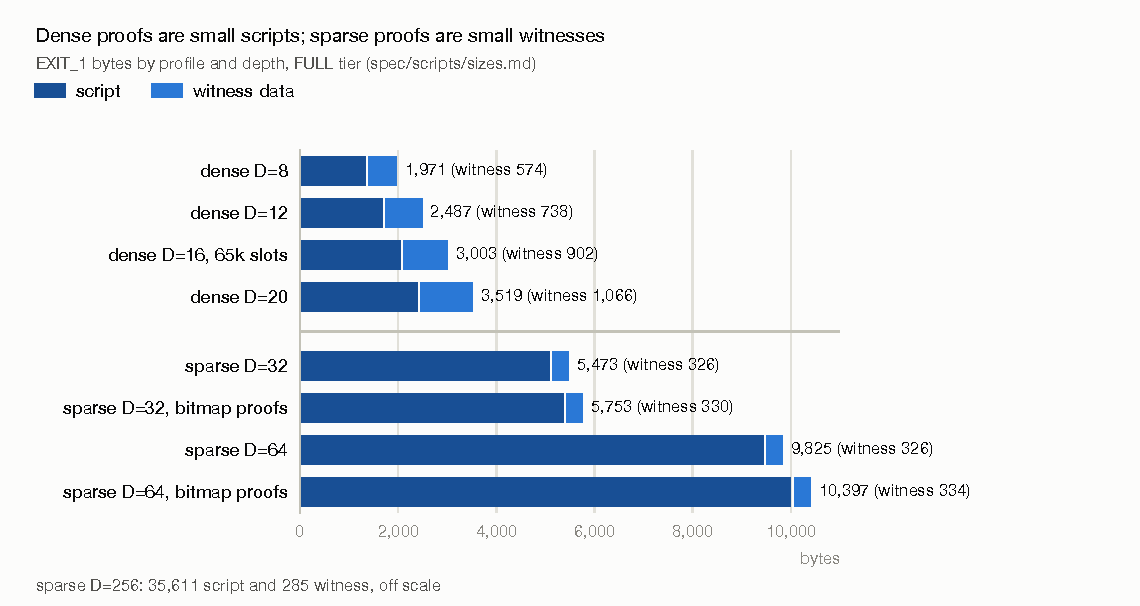
\includegraphics[width=\linewidth]{figures/exit-profiles.pdf}
\caption{\tr{EXIT}$_1$ bytes by profile and depth, FULL tier: dense
proofs are small scripts, sparse proofs small witnesses. Sparse rows are
measured on the six-leaf tree.}
\label{fig:cmp-profiles}
\end{figure}

Dense is therefore the default (spec~5.4, \path{spec/layertree.md}):
1.7 to 2.8 times cheaper per exit at $2^{16}$ members, with cohort grafts
at one price, sweeps at about $160\vB$ per leaf and every batch shape, at
the price of an operator who keeps the slot map. The sparse profile is kept,
specified and tested as the measured alternative, and for deployments that
are key-addressed registries.
